\documentclass[11pt,a4paper]{article}
\usepackage[margin=2.5cm]{geometry}
\usepackage{amsmath,amssymb,booktabs,graphicx,url,microtype}
\usepackage[hidelinks]{hyperref}
\title{When Better Candidates Hurt Search: Paired Counterfactual Audits of Candidate Replacement in Differential Evolution, Particle Swarms and CMA-ES}
\author{Alan Vallavaraj}
\date{Research manuscript draft, 23 September 2026}
\begin{document}
\maketitle
\begin{abstract}
Candidate-interception methods can substitute an optimizer's next proposed point without increasing that optimizer's online evaluation budget. I ask whether a replacement with a lower immediate objective value improves the optimizer after an equal continuation budget. At each checkpoint I copy the complete state of differential evolution (DE), particle swarm optimization (PSO), or covariance matrix adaptation evolution strategy (CMA-ES), evaluate the original or transformed point in separate branches, and then continue each branch without intervention under matched random streams. Across 24 noiseless COCO/BBOB functions, dimensions 5, 10 and 20, two instances and two seeds per dimension, contraction gave an immediately better candidate in 267 DE, 257 PSO and 240 CMA-ES forks. Despite that improvement, the transformed branch later had worse best-so-far fitness in 48/267, 26/257 and 134/240 forks, respectively. On unused BBOB instance IDs, a 576-checkpoint CMA-ES audit found delayed harm after 208/478 immediately better candidates under direct replacement and 211/478 under the documented \texttt{inject()} interface. Injecting was better than direct replacement in 277 continuations, worse in 273 and tied in 26. The diagnostic forks themselves require additional real evaluations. These findings establish a failure mode for immediate candidate-quality proxies in the tested settings, and motivate trajectory-aware validation of candidate-interception methods; they do not identify an optimizer that consistently outperforms published methods.
\end{abstract}

\noindent\textbf{Keywords:} black-box optimization; causal intervention; CMA-ES; differential evolution; particle swarm optimization; BBOB; reproducible benchmarking.

\section{Introduction and related work}
Surrogate-assisted optimization often proposes candidates before expensive evaluation. Classical response-surface and infill approaches include efficient global optimization, its taxonomy, online approximations and multiobjective extensions \cite{jones1998ego,jones2001,knowles2006,zhang2010}. Approximate fitness, surrogate-assisted evolutionary computation and surveys examine the risks of prediction error and limited evaluation budgets \cite{jin2002,jin2011survey,haftka2016,stork2020}. The surrogate may filter or replace proposed points and alter the future algorithm state. Generic wrappers and probabilistic surrogate frameworks make such replacement possible across hosts \cite{ong2003,lim2010,cai2020,blank2021psaf,gpsaf2022}. Thus generic candidate interception itself is established.

Applications and alternative mechanisms span dynamic optimization, data-driven constrained systems, local/global metamodels, robust design and parameter control \cite{luo2019,wang2020forest,zhou2007,ong2006,bagheri2017}. Evolution-strategy surrogates and metamodel-assisted preselection provide additional host-specific precedents \cite{emmerich2002,hansen2019surrogate}. Differential evolution and swarm optimization admit classification-assisted replacement, cooperative search, active learning and multiple local surrogates \cite{lu2011,wang2019de,sun2017pso,lv2019,wang2017committee,li2021}. Expensive many-objective work uses classification, decomposition, constraints and parallel infill; these are relevant to the scope of candidate selection, although our experiments have one objective and no constraints \cite{habib2019,pan2019,deb2019taxonomy,viana2010,beaucaire2019,berveglieri2020,bagheri2017constraint}. Widely used implementation platforms are described in \cite{blank2020pymoo,tian2017}.

The hosts draw on the original DE, PSO and CMA-ES designs \cite{storn1997,kennedy1995,hansen2001}. Hansen explicitly described external-solution injection and step renormalization in CMA-ES \cite{hansen2011inject}. Contemporary work on budget-neutral geometry-guided infill and on delayed lineage value further narrows any originality claim concerning candidate modification or long-horizon credit \cite{yu2026janus,siper2026}. This study contributes an empirical measurement of how often an \emph{actually better evaluated candidate} fails to improve the later trajectory in three specified host implementations, plus a fresh-instance comparison of direct CMA-ES replacement with native injection. This is an evaluation study rather than a new optimization algorithm.

\section{Methods}
\subsection{Paired state-clone contrast}
For minimization, let $S_t$ denote the complete host state and $x_t$ its next proposal. A treatment transforms $x_t$ into $T(x_t,S_t)$; PASS evaluates the original. I clone the host and its random state before proposal, evaluate exactly one point in each branch at the intervention step, and then run $H-1$ ordinary host evaluations in each branch. Both branches therefore have the same continuation budget, while producing both branches for diagnosis costs additional true evaluations. Define
\begin{equation}
\delta_1=f(x_t)-f(T(x_t,S_t)),\qquad
\Delta_H=b_{t+H}^{\mathrm{PASS}}-b_{t+H}^{T},
\end{equation}
where $b$ is best-so-far objective value. Conditional harm is $\Delta_H<-10^{-9}$ among checkpoints with $\delta_1>10^{-9}$. This compares the \emph{candidate} immediately, not necessarily a new incumbent. PASS candidate fitness is observed only in the diagnostic experiment and is not available for free to a live decision policy. Common random numbers improve precision without forcing the subsequently diverged trajectories to have identical proposals.

Two fixed transformations are studied: contraction $T_C(x)=\operatorname{clip}\{x+0.45(x_{\mathrm{best}}-x)\}$ and step reflection $T_R(x)=\operatorname{clip}\{x_{\mathrm{parent}}-0.75(x-x_{\mathrm{parent}})\}$. The clip uses the problem bounds. DE uses rand/1/bin, $F=0.7$, crossover probability $0.9$ and elitist parent replacement. PSO uses inertia $0.7$, cognitive and social coefficients $1.4$ and a global best. The PSO treatment changes the particle's position and velocity. CMA-ES uses \texttt{cma} 4.5.0 ask/tell, center initialization, an initial step size $0.3$ times average box width and population $\max(8,\lfloor4+3\log D\rfloor)$; the other hosts use $\max(8,5D)$ individuals. These are defined host implementations rather than claims about all DE, PSO and CMA-ES variants.

\subsection{Benchmark and evaluation accounting}
COCO's noiseless BBOB suite comprises 24 functions; multiple instances change underlying shifts and transformations \cite{hansen2009bbob,hansen2020coco}. I use all 24 functions at $D\in\{5,10,20\}$, two instances and two seeds per dimension. Main experiment suite indices 6--7, 8--9 and 12--13 correspond to actual instance IDs 71--72, 73--74 and 77--78. Each baseline uses $20D$ true evaluations; each of PASS, contraction and reflection uses a further $20D$. This gives 288 checkpoint states per dimension, 864 branch rows per dimension, and $806{,}400$ true evaluations over the three dimensions. A regression check copies PASS twice and verifies identical first and subsequent objectives on a test problem.

The cap check has separate instance IDs 75--76, two seeds and 96 checkpoints at each of 5D and 10D. The displacement from an original proposal to its contracted proposal is capped at $0.5\sqrt D$ Mahalanobis units under the current CMA-ES search distribution. This is a specific fixed cap, not a replication of the entire injection method of \cite{hansen2011inject}. PASS, contraction and capped contraction receive identical $20D$ branch budgets. The two checks add $115{,}200$ true evaluations.

An additional CMA-ES audit uses unused instance IDs 79--80, four seeds, all 24 functions and three dimensions. Checkpoints occur after 104, 200 and 408 evaluations respectively, at complete generation boundaries. Each state produces PASS, direct replacement in \texttt{tell()}, and \texttt{CMAEvolutionStrategy.inject([genotype], force=True)} before \texttt{ask()}. The bounded candidate is converted back to genotype with the library boundary inverse. The two treated branches evaluate the same first candidate within floating-point tolerance; native injection can change subsequent assignment of common random variates to samples. The continuation is $20D$ evaluations without further treatment. The 576 checkpoints yield 1,728 branch rows and $539{,}904$ true calls including baseline and branches.

Function-cluster bootstrap intervals resample the 24 functions, preserving the within-function dependence of instance and seed repetitions. These are descriptive uncertainty intervals for the specified benchmark design, not coverage guarantees for unseen real-world functions. All counts and interval computations are regenerated by the released scripts.

\section{Results}
\subsection{Contraction and reflection}
\begin{table}[ht]
\centering\small
\caption{Harmful later best-so-far outcome conditional on an immediately better contraction candidate. Fractions show harm / immediately better candidates; hosts need not visit the same states.}
\label{tab:main}
\begin{tabular}{lrrr}\toprule
Dimension & DE & PSO & CMA-ES\\\midrule
5 & 18/87 (20.7\%) & 8/77 (10.4\%) & 41/80 (51.3\%)\\
10 & 18/89 (20.2\%) & 10/88 (11.4\%) & 47/79 (59.5\%)\\
20 & 12/91 (13.2\%) & 8/92 (8.7\%) & 46/81 (56.8\%)\\\midrule
Pooled descriptive & 48/267 (18.0\%) & 26/257 (10.1\%) & 134/240 (55.8\%)\\\bottomrule
\end{tabular}
\end{table}
\begin{figure}[ht]\centering
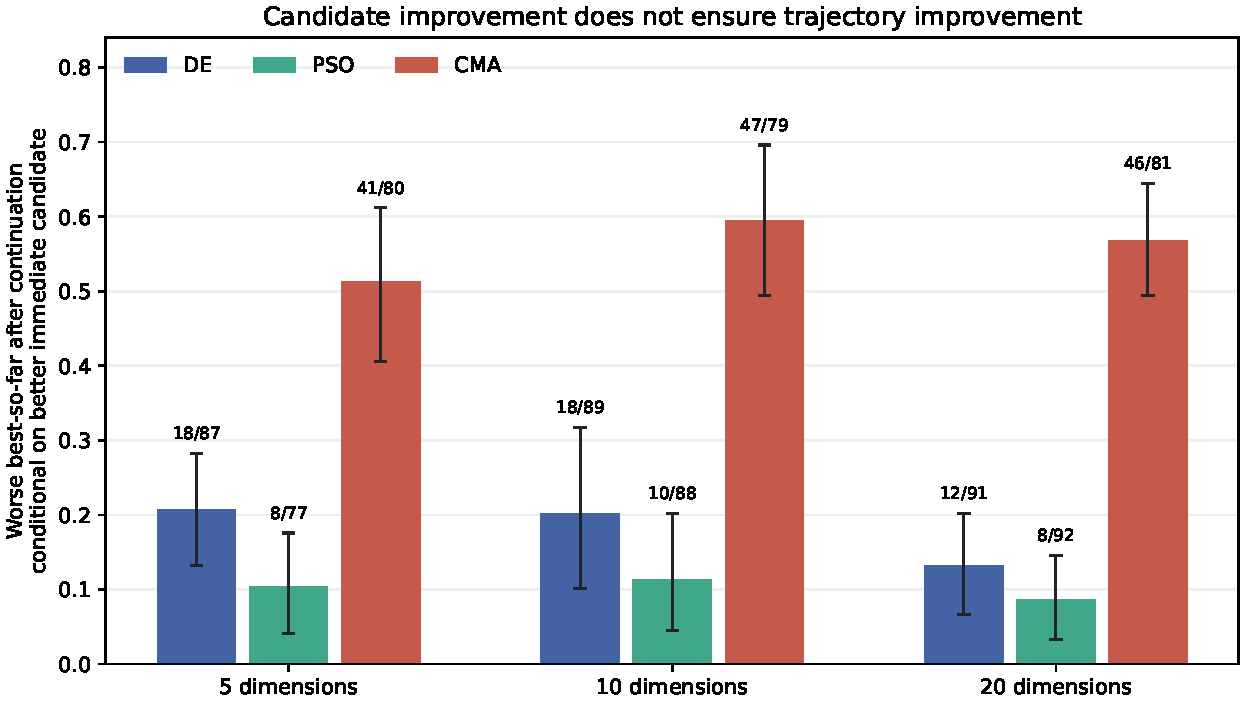
\includegraphics[width=.86\linewidth]{figures/fork_conditional_harm.pdf}
\caption{Conditional contraction harm by dimension. Intervals resample functions as clusters.}\label{fig:host}
\end{figure}
Reflection gives fewer immediately better proposals: descriptive pooled conditional harm is 7/108 in DE, 1/45 in PSO and 59/104 in CMA-ES. The function-cluster mean harm-rate difference (CMA-ES minus DE) for contraction is 0.281 (95\% bootstrap interval 0.170--0.389) in 5D, 0.410 (0.246--0.562) in 10D, and 0.448 (0.340--0.552) in 20D. These are between-host associations under different visited states, populations and proposals; they do not isolate the covariance update as the cause.

The fixed cap beats/loses/ties against uncapped contraction in 14/17/65 five-dimensional forks and 2/6/88 ten-dimensional forks. It changes the first candidate's value in only 31/96 and 8/96 forks respectively. This cap was often inactive and did not resolve the observed harm; stronger conclusions about injection safeguards do not follow.

\subsection{Fresh-instance injection audit}
\begin{table}[ht]\centering\small
\caption{Fresh-instance CMA-ES audit. Harm is conditional on the direct and injected branches sharing an immediately better first candidate.}
\label{tab:inject}
\begin{tabular}{rrrrr}\toprule
$D$ & Checkpoints & Better first & Direct harm & Inject harm\\\midrule
5 & 192 & 161 & 74/161 (46.0\%) & 65/161 (40.4\%)\\
10 & 192 & 153 & 63/153 (41.2\%) & 66/153 (43.1\%)\\
20 & 192 & 164 & 71/164 (43.3\%) & 80/164 (48.8\%)\\\midrule
Pooled & 576 & 478 & 208/478 (43.5\%) & 211/478 (44.1\%)\\\bottomrule
\end{tabular}\end{table}
\begin{figure}[ht]\centering
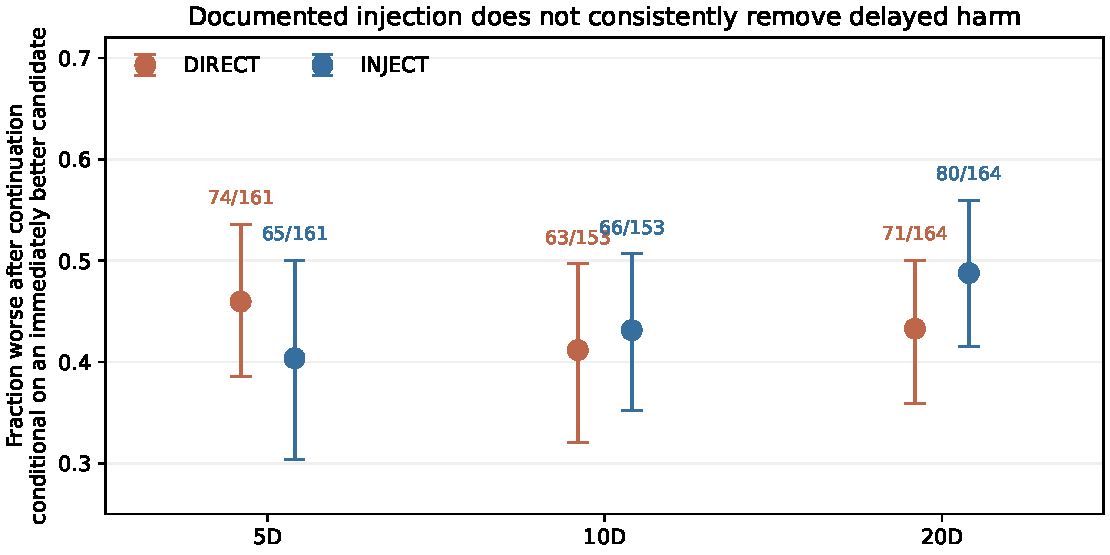
\includegraphics[width=.86\linewidth]{figures/injection_harm_comparison.pdf}
\caption{Delayed harm for direct and native injection across fresh instances. Intervals resample functions.}\label{fig:inject}
\end{figure}
The equal-function mean difference in conditional harm (direct minus injected), pooled descriptively over dimensions, is $-0.002$ with function-cluster bootstrap interval $[-0.054,0.053]$. Injection wins/loses/ties against direct treatment in 277/273/26 checkpoints. This evidence does not show consistent rescue by the native interface under the tested contraction source. The documented interface may still protect against different external candidates or instabilities. Recorded mean shift, step-size ratio and covariance ratios after the first generation do not isolate one decisive mechanism; direct and injected branches also differ in later proposal assignment.

\section{Limitations and implications}
The within-host PASS-versus-treatment branch difference is a causal contrast at each cloned checkpoint for the specified one-time transformation and continuation. The conditional harm rate is selected by the observed immediate candidate difference; it is a diagnostic rate and does not evaluate a deployable gate. Host comparisons are not randomized across identical state distributions. Only deterministic, box-constrained, noiseless benchmark problems, two transformations, basic hosts and one continuation horizon were evaluated. Fresh injection instances test a new indexing and seed regime on the \emph{same} 24 function definitions, not a wholly independent function suite. Diagnostic computation is much larger than the online budget of one branch. Neither a deployable improvement policy nor state-of-the-art optimization performance has been demonstrated.

A submission claiming practical optimizer improvement would require independently implemented hosts, stronger new problem distributions, more configurations and noise, target-based and anytime COCO metrics, measured online budgets, and comparisons against established surrogate and injection methods. Controlled ablations would be required to distinguish covariance adaptation from different proposed points and other host-state effects. The current data support a narrower contribution: immediately better candidate quality is an unreliable proxy for later trajectory value in these specified conditions. Complete branch trajectories, fixed scripts and instructions accompany the manuscript for independent checking.

\section*{Data and code availability}
The public repository \url{https://github.com/alanvallavaraj/candidate-intervention-trajectory-audit} provides scripts, raw branch CSVs, generated analyses, PDF figures, dependencies and exact reproduction commands. No external human or patient data were used. Affiliation and any journal-specific declarations must be supplied by the author before submission.

\bibliographystyle{unsrt}
\bibliography{references}
\end{document}
